\section{Data preprocessing}
\label{section:Data:Preprocessing}
This section briefly describes all the data processing done.

\subsection{Feature generation}
Both the feature \textit{"hits"} and \textit{"clicks"} can be argued to measure
user interest. A products hits score measure how many times someone has clicked
on to that product information page at prisuigen.no. A products click score measure
how many times prisguiden.no has redirected an user to an external retailer for the given product.
We ended up combining these two variables into one feature which we called \textbf{"interest"}
with the equation defined in \Cref{eq:interest}.
\begin{equation}
  interest = hits + clicks
  \label{eq:interest}
\end{equation}

\subsection{Value Scaling}
For the neural net models we scale using normalization for the ranges to be in the range [0.1, 1].
The unconventional choise of having 0.1 as our lower bound is becuase the matric SMAPE
is vulnerable to zero values, as described in \Cref{eq:sMape}.
Normization was chosen over standardization because we do not know the distrubtion
of the data, and we did not want to assume it followed a Gaussion distribution.
All model output and predictions are rescaled to it's original range before
visualizing and plotting.

For the ARIMA models we did not scale the data because ARIMA models will not
get the same benefits by scaling the input data.

%The way our data pipeline was constructued made it self documenting,
%which means it prints out all the processing steps and saves them as the
%experiment is conducted. This section will briefly cover how the data was processed
%before each type of experiments.
%The different model structures required some differences in processing steps.

\subsection{Univariate to Multivariate feature engeneering}
Since the E-commerce domain is heavily influenced by external factors, such as
holidays, Christmas, and yearly seasons we thought it would be beneficial
for the neural net models to be aware of which day of the week it is,
which month it is, and if it is closer to summer than winter.

We add the \textit{month} feature, a number between [0, 11] depending on which month.

We add the \textit{day} feature, a number between [0, 6] where 6 is saturday, 0 is sunday etc.
We can calculate the day of the week using the formula \Cref{eq:day_of_the_week}
from \Cref{section:BT:day-of-the-week-formula}.

We add the feature \textit{season} which is a number between [-1, 1] using \Cref{eq:season_feature}.

\begin{equation}
  season = \cos(\pi * (month \mod{12}) / 6)
  \label{eq:season_feature}
\end{equation}

\begin{figure}[h!]
  \centering
  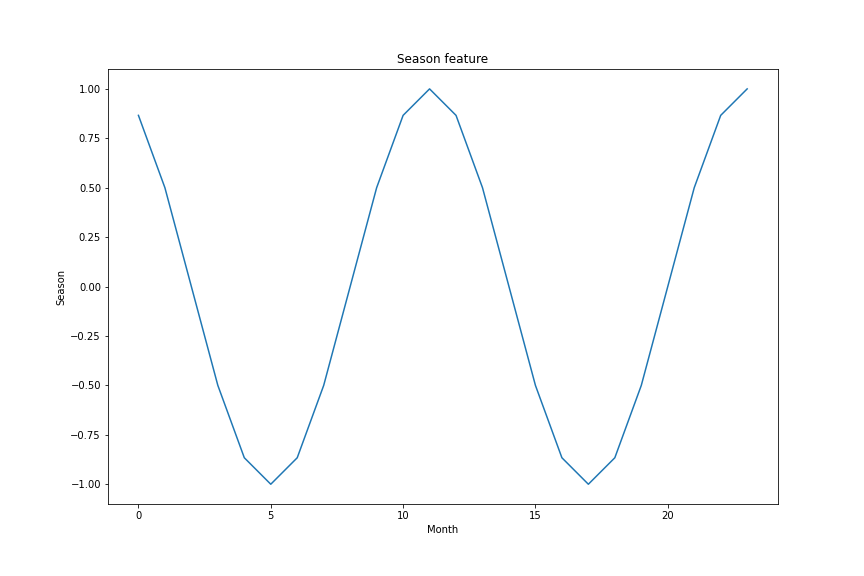
\includegraphics[width=\textwidth]{./figs/code_generated/season_feature.png}
  \hfill
  \caption{Season feature}
  \label{fig:season-feature}
\end{figure}

\Cref{fig:season-feature} shows the output of the season feature.
If the month is close to Christmas (december, januar) this feature will be close to 1.
If the month is closer to summer (may, june) this feature will be close to -1.

In the and all added features are scaled between [0.1, 1] as described above.

\subsubsection{Moving Window Approach}
We are using the same approach  as in \cite{Bandara2019} %Sales Demband FOrecast in E-commerce
and \cite{Hewamalage2021}% Current state and future predictions
\todo[inline]{Write this section.}
\begin{figure}[h!]
  \centering
  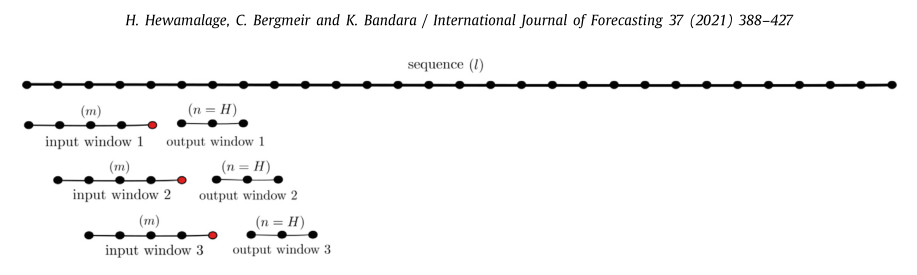
\includegraphics[width=\textwidth]{./figs/illustrations/moving_window_illustration.png}
  \hfill
  \caption{Moving window scheme \citep{Hewamalage2021}}
  \label{fig:dataset:moving_window_scheme}
\end{figure}

\subsection{Train, validation, test splitting}
TODO: